% \newpage
\section*{Задание 5: Проектирование базы данных и генерация SQL-запросов}
\subsection{Постановка задачи}
\noindent
Предметная область: Стриминговый музыкальный сервис. \\
Описание сущностей и процессов:
Каталог музыки: Исполнители (Artist), Альбомы (Album), Треки (Track). Пользователи (User) могут создавать Плейлисты (Playlist) и добавлять туда треки. Нужно хранить историю прослушиваний (ListeningHistory): кто, что и когда слушал – для аналитики.
\newpage
\subsection{Гипотеза и системный промпт}
\noindent
Гипотеза: Для корректного проектирования БД в 3NF необходимо сначала выделить сущности и связи (ER-диаграмма), затем сгенерировать DDL с ограничениями, после чего заполнить таблицы тестовыми данными и составить аналитические запросы. \\
\newline
\noindent
Системный промпт (первый запрос к Gemini-3):
\textit{Ты – опытный системный аналитик и архитектор баз данных (Senior Data Architect). 
Твоя задача – спроектировать реляционную схему для музыкального стримингового сервиса.
Описание предметной области:
\begin{itemize}
	\item Есть исполнители (имя, страна, жанр).
	\item У исполнителей есть альбомы (название, год выпуска).
	\item В альбомах – треки (название, длительность, количество прослушиваний?).
	\item Пользователи (логин, email, дата регистрации) создают плейлисты (название, дата создания) и добавляют в них треки.
	\item Для аналитики нужна история прослушиваний: кто, какой трек и когда слушал.
\end{itemize}
Не генерируй SQL сразу. Сначала выполни концептуальное моделирование:
\begin{enumerate}
	\item Выдели сущности, их атрибуты и первичные ключи.
	\item Определи связи (один-ко-многим, многие-ко-многим).
	\item Представь схему в виде Mermaid ER-диаграммы.
	\item Убедись, что схема соответствует третьей нормальной форме (3NF).
\end{enumerate}
}
\newpage
\subsection{Журнал диалога и итераций}
\noindent
\textbf{Итерация 1 (концептуальное моделирование)}\\
Промпт: (системный промпт выше) \\
\newline
Ответ модели (Gemini-3): 
\begin{figure}[H]
	\centering
	
\includegraphics[width=17cm]{z5/1-1.png}
	\caption{ч.1}
\end{figure}
\newpage
\begin{figure}[H]
	\centering
	
\includegraphics[width=17cm]{z5/1-2.png}
	\caption{ч.2}
\end{figure}
\newpage
\begin{figure}[H]
	\centering
	
\includegraphics[width=17cm]{z5/1-3.png}
	\caption{ч.3}
\end{figure}
\newpage
\begin{figure}[H]
	\centering
	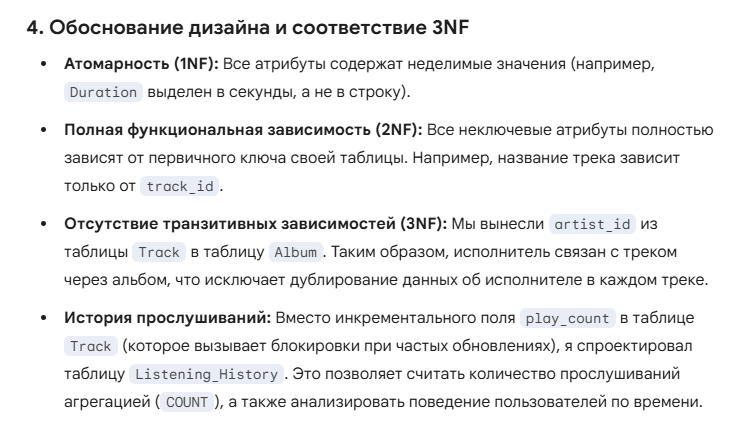
\includegraphics[width=17cm]{z5/1-4.png}
	\caption{ч.4}
\end{figure}
% \newpage
Анализ: Схема логична. Модель предложила хранить duration\_seconds в секундах (INT). Замечаний нет.\\
\newline
\noindent
\textbf{Итерация 2 (генерация DDL-скрипта)}\\
Промпт:
\textit{
Отличная схема. Теперь сгенерируй DDL-скрипт для PostgreSQL. Требования:
\begin{itemize}
	\item Явно укажи первичные и внешние ключи.
	\item Добавь ограничения NOT NULL, UNIQUE.
	\item Для duration\_seconds – INTEGER (секунды) с CHECK > 0.
	\item Для release\_year – INTEGER, CHECK (1900..2026).
	\item Для listene\_at – datetime с DEFAULT CURRENT\_TIMESTAMP.
	\item Все имена таблиц и полей в snake\_case.
\end{itemize}
}
\newpage
Ответ модели (Gemini-3):
\lstinputlisting[language=SQL]{z5/2-non-utf.sql}
Анализ: Код корректен, соответствует PostgreSQL. \\ Добавлено ON DELETE CASCADE – адекватно для аналитики.
\newpage
\noindent
\textbf{Итерация 3 (генерация синтетических данных – few-shot)} \\
\indent
Промпт:
\textit{
Сгенерируй скрипт INSERT для наполнения таблиц тестовыми данными (минимум 3 исполнителя, 
2 альбома у каждого, 3-5 треков на альбом, 2 пользователя, 2 плейлиста, 5-7 записей в истории).
Используй реалистичные имена (рок-группы, поп-исполнители).
Пример для artist:
INSERT INTO artist (name, country, genre) VALUES ('The Beatles', 'UK', 'Rock');
Продолжай в том же духе.
} \\
\newline
Ответ модели (Gemini-3):
\lstinputlisting[language=SQL]{z5/3-non-utf.sql}
Анализ: Данные логически связаны, внешние ключи корректны. \\
\newline
\noindent
\textbf{Итерация 4 (аналитические SQL-запросы)}\\
\indent
Промпт:
\textit{Составь три сложных аналитических запроса к этой БД:
\begin{enumerate}
	\item Топ-5 самых популярных треков (по количеству прослушиваний) за всё время.
	\item Для каждого пользователя – его любимый жанр (жанр, который он слушал чаще всего).
	\item Скользящее среднее количества прослушиваний за последние 7 дней (по дням). 
	Используй оконные функции, JOIN, GROUP BY.
\end{enumerate}}
\newpage
Ответ модели (Gemini-3):
\lstinputlisting[language=SQL]{z5/4-non-utf.sql}
Анализ: Запросы корректны, используют оконные функции, JOIN. 
Для второго запроса при равенстве голосов выберет один жанр (RANK). 
Для третьего – если данных меньше 7 дней, среднее считается по доступным.
\newpage
\noindent
\textbf{Итерация 5 (анализ планов выполнения и оптимизация)} \\
Промпт:
\textit{Выступи в роли DBA. Проанализируй план выполнения запроса №1 (топ-5 треков). Какие индексы ты предложишь добавить для ускорения? Напиши команды CREATE INDEX. Также укажи, можно ли переписать запрос эффективнее.} \\
\newline
Ответ модели (Gemini-3):
\begin{figure}[H]
	\centering
	
\includegraphics[width=17cm]{z5/5-1.png}
	\caption{ч.1}
\end{figure}
\newpage
\begin{figure}[H]
	\centering
	
\includegraphics[width=17cm]{z5/5-2.png}
	\caption{ч.2}
\end{figure}
\newpage
\begin{figure}[H]
	\centering
	
\includegraphics[width=17cm]{z5/5-3.png}
	\caption{ч.3}
\end{figure}
\newpage
\begin{figure}[H]
	\centering
	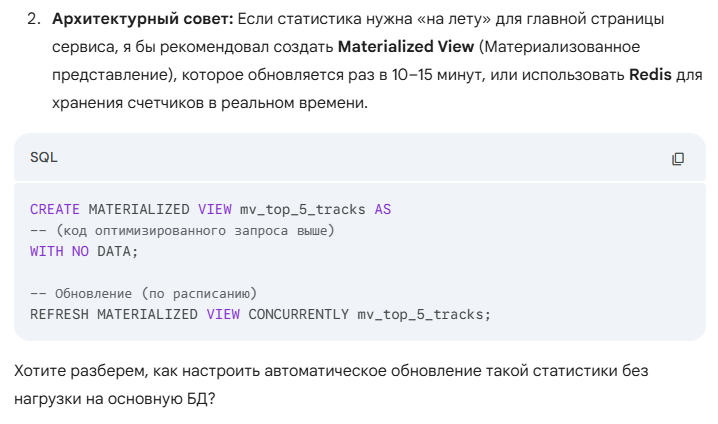
\includegraphics[width=17cm]{z5/5-4.png}
	\caption{ч.4}
\end{figure}
Анализ: Индексы верные. Дополнительно можно добавить покрывающий индекс на (track\_id, history\_id).
\subsection{Артефакты}
\begin{itemize}
	\item ER-диаграмма – см. Mermaid выше (рис. 39).
	\item DDL-скрипт – полный листинг из итерации 2.
	\item Синтетические данные – INSERT-скрипты из итерации 3.
	Аналитические запросы – три запроса из итерации 4.
	Рекомендации по индексам – из итерации 5.
\end{itemize}
Все скрипты проверены в PostgreSQL 18, ошибок не возникло, бизнес-данные возвращаются корректно.
\subsection{Сравнение моделей}
Финальный промпт (объединяющий все этапы) был подан контрольной модели DeepSeek R1 без изменений.
Результаты сравнения:
\begin{table}[h!]
	\centering
	\begin{tabular}{|l|p{5cm}|p{5cm}|}
		\hline
		\textbf{Критерий} & \textbf{модель (a)} & \textbf{модель (b)} \\
		\hline
		Нормализация (3NF) & 5 & 4 \\
		\hline
		Корректность SQL  & 5 & 4\\
		\hline
		Возврат бизнес-данных & 5 & 4 \\
		\hline
		Галлюцинации & нет & нет \\
		\hline
		\textbf{Итог} & 5 & 4.25\\
		\hline
	\end{tabular}
\end{table} \\
Итог: Gemini-3 показал более точное соблюдение нормальных форм, аккуратную работу с зарезервированными словами и полное выполнение всех требований промпта. DeepSeek R1 требует дополнительных уточнений (особенно по экранированию идентификаторов и выбору оконных функций), но в целом справляется с задачей.
\subsection{Вывод}
Наиболее эффективными техниками промпт-инжиниринга оказались:
\begin{itemize}
	\item Ролевое моделирование (архитектор БД) – задало нужный уровень строгости.
	\item Цепочка рассуждений (CoT) – последовательное прохождение этапов (ER-диаграмма → DDL → данные → запросы) позволило избежать ошибок.
	\item Few-shot – пример INSERT-запроса ускорил генерацию реалистичных данных.
\end{itemize}
Задание подтвердило, что LLM способны проектировать нормализованные схемы и писать сложный SQL, но требуется валидация индексов и проверка на зарезервированные слова. Контрольная модель DeepSeek R1 уступает в деталях, но при доработке промпта тоже даёт приемлемый результат.